%
%
%
\long\def\comment#1{}
\newif\ifcover

% \documentstyle[times,chi2003ea]{article}
% \documentclass[nocopyrightspace,times]{chiproceedings-nospace}
% \documentclass[nocopyrightspace]{chiproceedings-nospace}

% パタンはtt
% 出力文字列はsf

\documentclass{article}
\usepackage{times}
\usepackage{uist04}

\usepackage{here} % [H]とするとその場所に配置されるらしい

\long\def\ttt#1{\texttt{\small #1}}
\long\def\tsf#1{\textsf{\small{#1}}}
\long\def\tit#1{\textit{\small{#1}}}

\long\def\ST{\textsf{\small{Strotor}}}
\long\def\U{\textsf{\small{U}}}
\long\def\D{\textsf{\small{D}}}

\usepackage{graphicx}
% mediabb.sty というのを使うとPDFをそのままincludegraphicsできるらしい。
% http://www.ns.musashi-tech.ac.jp/~inoue/Pages/TeX/mediabb.sty.html
%
% \usepackage{mediabb}
% \usepackage{ascmac}

\begin{document}
\title{Strotor: A Minimalistic Approach to \\
Exploring Hierarchical Data}
\author{
\begin{tabular}{l}
\parbox{5.5cm}{
\begin{center}
Toshiyuki Masui\\
Keio University\\
masui@pitecan.com
~ \\
~ \\
~
\end{center}
}
\end{tabular}
}
\maketitle
\abstract
We introduce a new simple information navigation technique
that enables users to explore large hierarchical data structure
using only two keys or one rotating device that can generate
two different signals based on the rotation direction.
%
Using the rotation-based input device called ``\ST'',
users can find an entry in a huge hierarchical database easily
only by rotating a disk or a cylinder in two directions.
%
{\ST} can be easily installed in sofas, kitchens, cars, etc.
where standard keyboards and remote controllers do not fit.

\keywords Help systems, Approximate pattern matching, Generate-and-filter

\tolerance=400 
  % makes some lines with lots of white space, but 	
  % tends to prevent words from sticking out in the margin

\section*{INTRODUCTION}

Large data are often represented as a hierarchical data structure, and
various navigation methods are provided for exploring the data.
For example, files on Unix are structured hierarchically, and
various commands (\tsf{cd}, \tsf{ls}, etc.) and APIs are provided for exploring the file system.
Large dictionary database can also be treated as a large
hierarchical data, since the name of the entry can be treated hierarchically:
e.g. an entry for ``dictionary'' can be stored under ``d'' and ``d/i''.

Many information visualization techniques and navigation techniques
have been proposed for handling large hierarchical data.
On personal computers,
multiple GUI methods are provided for
exploring the hierarchical file structure, because
there is no best interaction technique for all the users and situations.
% there is no single interaction technique that is always good for any situation.

When a user cannot use a pointing device,
selection-based interaction techniques are used for
finding information in hierarchical data.
For example, a user can hierarchically find a music file by
selecting an artist from the list of artist names,
selecting an album title from the title list,
and selecting a music file from the song list.
% Users can do the selection jobs either by using a mouse or by using arrow keys.
% For exaple,
Users can use two keys for choosing an entry from the list
(e.g. selecting an artist from the artist list),
and often another key is used for selecting an entry and showing the next level
(e.g. selecting an artist and show album titles).
It is also necessary to provide a way to go back to the previous state, and
yet another key can be used for that task
(e.g. showing the artist list for artist selection).
%
This 4-way navigation is popular on small mp3 players\footnote{
  e.g. \textsf{http://www.iriver.com/product/view.asp?pCode=003\&pNo=37}
} and remote controllers like AppleRemote\footnote{\textsf{http://en.wikipedia.org/wiki/Apple\_Remote}}
for selecting a song from the hierarchical data.
4-way navigation is also available on desktop software like Finder.app on Mac.

\begin{figure}[H]
\centerline{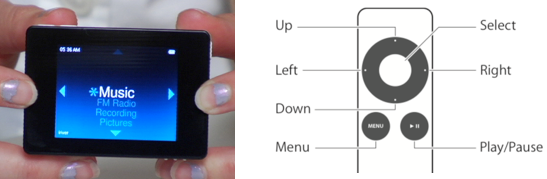
\includegraphics[width=80mm,bb=0 0 547 179]{figures/4buttons.png}}
\caption{4-button controllers on a small mp3 player and AppleRemote.}
\label{u10}
\end{figure}

% http://www.reigncom.com/eng/media/press/en_pr_read.asp?no_noti=1630&cd_noti_host=9
% D-Click Control System

% Small devices like Rio MP3 player and remote controllers like AppleRemote have
% 4 buttons for selecting a song from the hierarchical data.

Using 4 keys might be okay on these devices, but it would be much better
if we could perform the navigation task using only 2 keys.
In that case, we can use a rotating device like a disk or a cylinder for the navigation,
since the device can generate 2 signals based on the direction of the rotation (Figure \ref{rotation}).
%
% We have developed a new navigation technique where only two keys are required
% for exploring large hierarchical data, and implemented the system on
% a rotating device ``Strotor''.
%
We have developed a new navigation technique and device called ``{\ST}'',
where users can explore large hierarchical database by simple rotating operations.


% (語源)
% Navigating large structured data through rotation.

\begin{figure}[H]
\centerline{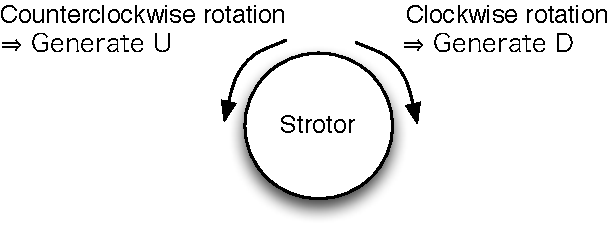
\includegraphics[width=60mm,bb=0 0 294 110]{figures/rotation.pdf}}
\caption{Using a rotation device for generating key events.}
\label{rotation}
\end{figure}

\section*{NAVIGATION METHOD AND EXAMPLES}

{\ST}'s behavior is based on the following simple principles.
Two types of operations, ``{\U}'' (up) and ``{\D}'' (down), are used for the navigation.
They can be generated either by rotating the {\ST} device or typing a keyboard.

\begin{enumerate}
\item A portion of the data is listed to the user.

\item One element in the list is selected and highlighted.

% \item Display the selected element, its siblings, its ancestors and their siblings.

\item When an elemented is selected, its siblings, its ancestors and their siblings are displayed
around the selected elememt.

\item Users can generate {\U} to select the element above the currently selected element,
or generate {\D} to select the element below the selected element.
Whenever the selection is changed, 3. is performed.
If the depth of the newly selected element is different from the currently
selected element, siblings of the currently selected element disappear.

\item When a newly selected element has children and the user performs no further action,
the first child of the selected elemented is newly selected, and 3. is performed.
As a result, all the siblings of the newly selected element
(the first child of the currently selected elmeent) appear in the list.

\end{enumerate}

We show how {\ST} works, using a hierarchical data structure of
shops list in a shopping mall shown in Figure \ref{fig1} as example data.
Rectangles with thick border represent categories, and
other rectangles represent individual shops.

\begin{figure}[H]
% 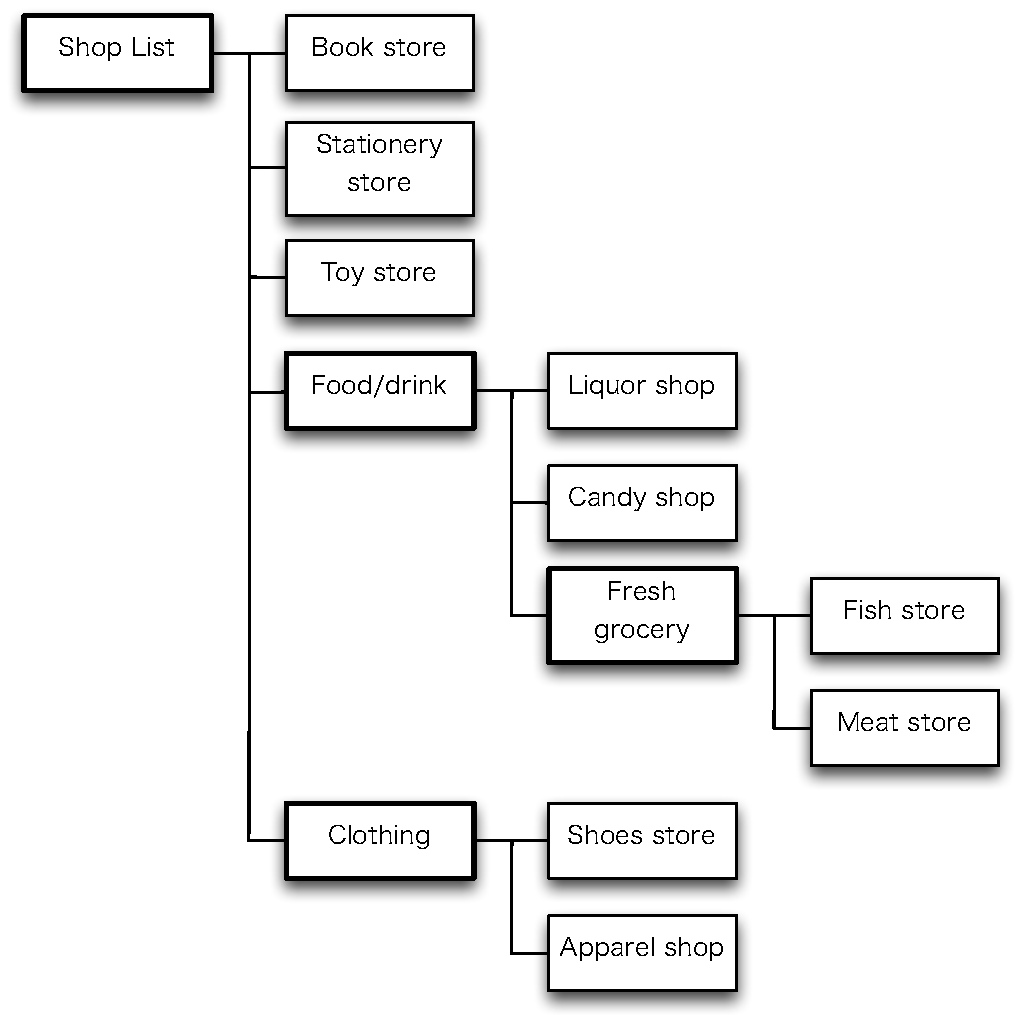
\includegraphics[width=70mm]{figures/fig1.pdf}
\centerline{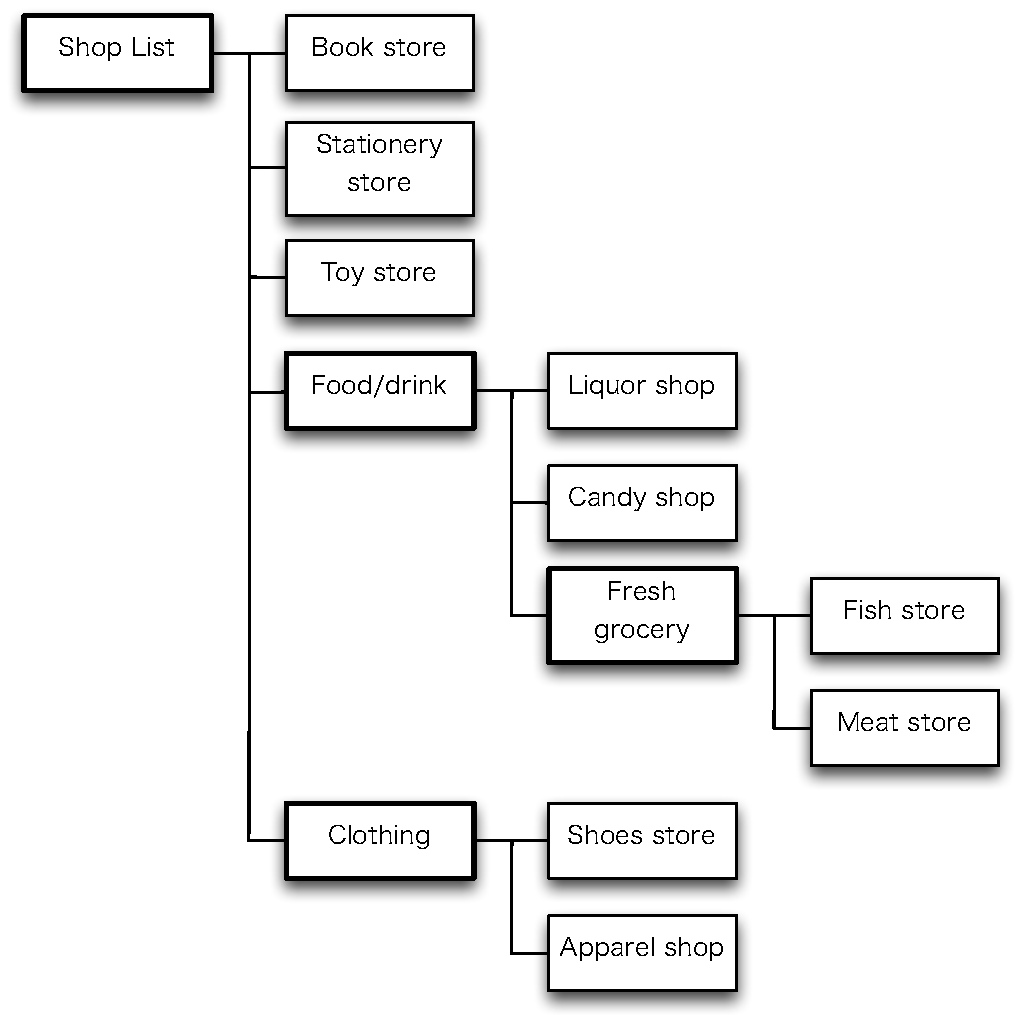
\includegraphics[width=80mm,bb=0 0 490 490]{figures/fig1.pdf}}
\caption{Sample data: shops in a shopping mall.}
\label{fig1}
\end{figure}

When the user starts the exploration, only the shops and categories
at the top level are displayed (Figure \ref{fig2}).
When the user generates {\D},
the second element (\tsf{Stationery store}) is selected (Figure \ref{fig3})\footnote{
  Readers can try this at \textsf{http://jsbin.com/lecuroku}.
}.

\begin{figure}[H]
\centerline{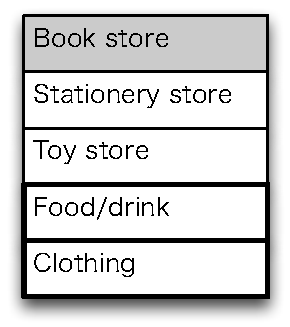
\includegraphics[width=24mm,bb=0 0 139 157]{figures/fig2.pdf}}
\caption{Initial display.}
\label{fig2}
\end{figure}

\begin{figure}[H]
\centerline{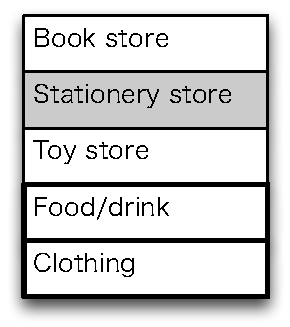
\includegraphics[width=24mm,bb=0 0 139 157]{figures/fig3.pdf}}
\caption{Typing {\D}.}
\label{fig3}
\end{figure}

If the user generates {\D} two more times, 
\tsf{Food/drink} category is selected (Figure \ref{fig4}).
If the user stops the operation and waits for a moment, the shops under the \tsf{Food/drink}
category are automatically displayed,
and the first entry (\tsf{Liquor shop}) is selected (Figure \ref{fig5}).

\begin{figure}[H]
\centerline{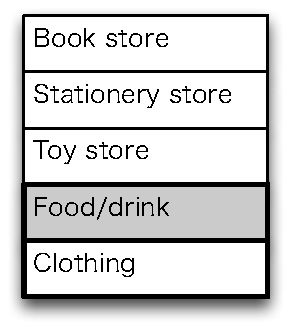
\includegraphics[width=24mm,bb=0 0 139 157]{figures/fig4.pdf}}
\caption{Selecting Food/drink.}
\label{fig4}
\end{figure}

\begin{figure}[H]
\centerline{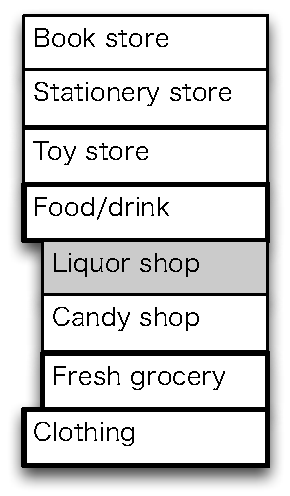
\includegraphics[width=24mm,bb=0 0 139 238]{figures/fig5.pdf}}
\caption{Selecting Liquor shop.}
\label{fig5}
\end{figure}

When the user generates {\D} twice,
\tsf{Fresh grocery} category is selected (Figure \ref{fig6}).

\begin{figure}[H]
\centerline{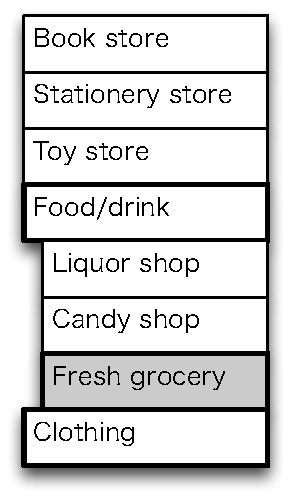
\includegraphics[width=24mm,bb=0 0 139 238]{figures/fig6.pdf}}
\caption{Selecting Fresh grocery.}
\label{fig6}
\end{figure}

If the user keeps generating {\D}, 
the list will change to Figure \ref{fig8},
without expanding the children of \tsf{Fresh grocery}.

\begin{figure}[H]
\centerline{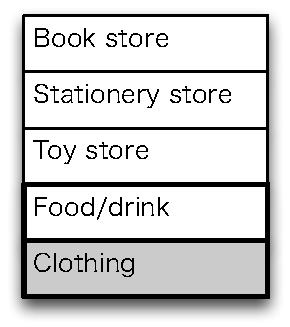
\includegraphics[width=24mm,bb=0 0 139 157]{figures/fig8.pdf}}
\caption{Selecting Clothing.}
\label{fig8}
\end{figure}

If the use stops generating {\D} at Figure \ref{fig6},
the shops under category \tsf{Fresh grocery} is automatically selected (Figure \ref{fig7}).

\begin{figure}[H]
\centerline{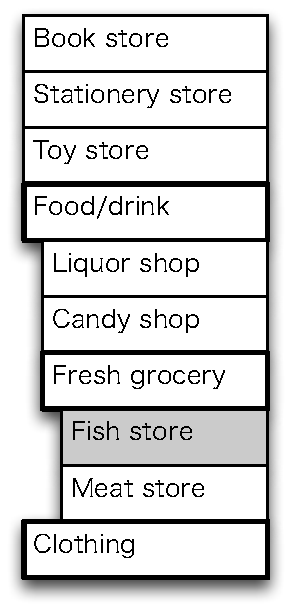
\includegraphics[width=24mm,bb=0 0 139 292]{figures/fig7.pdf}}
\caption{Selecting Fish store.}
\label{fig7}
\end{figure}

When the user generates {\U} here, \tsf{Fresh grocery} is selected,
and the shops under \tsf{Fresh grocery} disappears, 
resulting in the same state as Figure \ref{fig6}.
If the user generates {\U} two more times, the display changes to the state
shown in Figure \ref{fig5},
and one more {\U} will set the system to the state of Figure \ref{fig4}.

If the user generates {\D} in Figure \ref{fig4}, the next visible entry
(\tsf{Clothing}) is selected (Figure \ref{fig8}), and then the state changes to Figure \ref{fig9}.

\begin{figure}[H]
\centerline{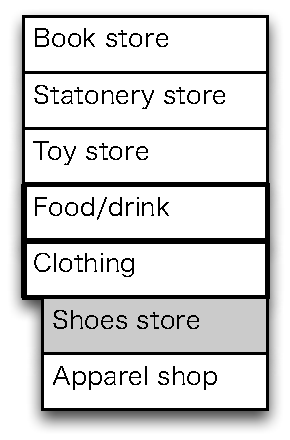
\includegraphics[width=24mm,bb=0 0 139 211]{figures/fig9.pdf}}
\caption{Selecting Shoed store.}
\label{fig9}
\end{figure}

When the user generates {\D} twice in Figure \ref{fig7},
\tsf{Clothing} is selected, and the category will be expanded (Figure \ref{fig8}).

In this way, users can explore the hierarchical structure
only by generating {\U}/{\D} keys at the right timing.

\section*{Implementation}

A prototype system was built using JavaScript and it runs on modern browsers.
A large list of news articles, movies, anime films, musics, and e-book titles are listed in one browser window
and the content is displayed in another window (Figure \ref{screenshot}).

\begin{figure}[H]
\centerline{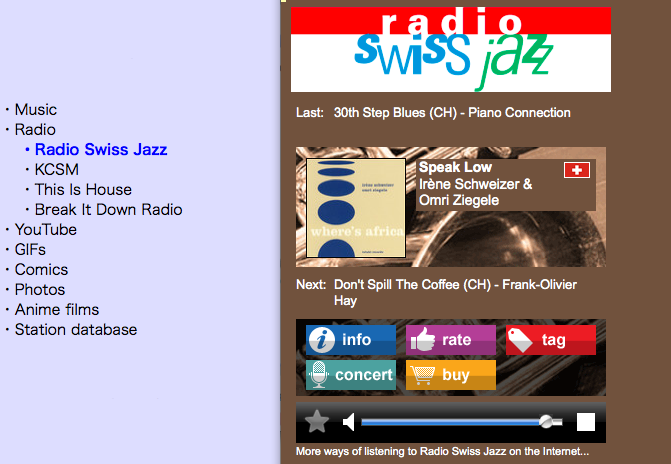
\includegraphics[width=80mm,bb=0 0 671 464]{figures/95cf2fec71c52ead6fdbcb7f79aca654.png}}
\caption{Selecting an Internet radio station.}
\label{screenshot}
\end{figure}

We used
PowerMate\footnote{
  \textsf{http://griffintechnology.com/support/powermate}
} from Griffin Technology for the rotating device.
PowerMate generates standard keyboard events when rotated,
and no special programming techniques are required.
%
Users can explore all the contents just by
rotating the device clockwise and counterclockwise.

\begin{figure}[H]
\centerline{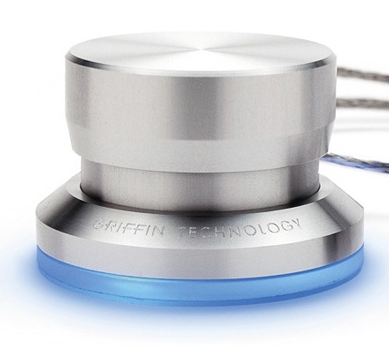
\includegraphics[width=30mm,bb=0 0 389 348]{figures/d3a69499f7e7314ae6dc10f5bf3a2be5.png}}
\caption{A PowerMate used for the prototype.}
\label{powermate}
\end{figure}

\section*{DISCUSSIONS}

\subsection{Comparison with existing methods}

4-way navigation are quite common for exploring hierarchical data structure,
and it is familiar to computer users.
Some mobile phones and PDAs are equipped with a jog dial with a push button,
where the dial is used for choosing an item from a list and 
the push button is used for fixing the selection.
% PowerMate is equipped with a push button which can used for such purposes.
% As far as we know,
All the existing methods require more than 2 keys/buttons, and
to the best of the authors' knowledge,
{\ST} is the only interaction method for exploring hierarchical data structure
with one rotating device.

Using a conventional hierarchical menu,
child elements are displayed automatically when their parent element is selected by a mouse.
The behavior is common to computer users,
and {\ST}'s automatic transition (e.g. from Figure \ref{fig4} to Figure \ref{fig5})
looks familiar to users.

\subsection{Comparison with InfoVis techniques}

Various information visualization techniques like
Treemap\cite{Johnson:1991:TSA:949607.949654},
Hyperbolic Tree\cite{Lamping:1995:FTB:223904.223956},
and Sunburst\cite{Stasko:2000:FDN:857190.857683}
have been proposed for visualizing large hierarchical data.
Zooming user interface (ZUI) systems like
Pad\cite{Perlin:1993:PAA:166117.166125} and
Pad++\cite{Bederson:1994:PZG:192426.192435}
can also been used for handling large hierarchical data laid out on a 2D space.
%
These visualization techniques and descendent technologies have become popular these days and
all of these systems are useful for understanding the structure of
large hierarchical data, but users of these systems have to use a pointing device
to take full advantage of their advantages.

% More conventional visualization techniques like TreeView\footnote{
%   \textsf{http://en.wikipedia.org/wiki/Tree\_view}
% } by replacing 4-way navigation to our approach.

% {\ST} can be adopted to more conventional visualization techniques like
% TreeView\footnote{
%   \textsf{http://en.wikipedia.org/wiki/Tree\_view}
% } by replacing 4-way navigation to our approach.

It seems to be a good idea to use {\ST} on more conventional visualization techniques like
TreeView\footnote{
  \textsf{http://en.wikipedia.org/wiki/Tree\_view}
}, by replacing 4-way navigation to {\ST}.

% LensBar\cite{Masui:1998:LVB:647341.721215}
% is also a ZUI system for handling large hierarchical data,
% but the same data structure used in LensBar can be used for {\ST}.
% Users can use a pointing devices when it is appropriate,
% and use two keys or a disk device when pointing devices is not available.

\subsection{Timing control}

The biggest disadvantage of {\ST} is that
the behavior of {\ST} depends on the speed of the user's operations.
In Figure \ref{fig4},
if a user wanted to select \tsf{Clothing} but couldn't generate {\D}
quickly enough, he will see Figure \ref{fig5} instead of Figure \ref{fig7}.
This is a tradeoff between usability and simplicty, and
the best parameter should be set based on the user and the {\ST} device.

\section*{EVALUATION}

No formal evaluation have been done yet, but {\ST} has been used in the author's
living room for six months, and the author's family members are using it
everyday for watching anime films and listening to music.
Besides PowerMate, a wireless mouse is preferred,
since we can carry a wireless mouse anywhere and select
a film or a music just by rotating the mouse wheel.

We displayed {\ST} at an exhibition
held in November 2013, and asked more than 100 people to try it
(Figure \ref{exhibition}).
%
Since the only thing a user can do with {\ST} is to rotate the device,
users seemed to be able to understand the behavior of {\ST} with trials and errors.
% 
% a user can use the device and see what happens without thinking about
% other interactions.
% 
Using only one rotating device for data navigation is a new experience for
all the subjects, but the hard restriction of the device seems to have worked in this case.

\begin{figure}[H]
\centerline{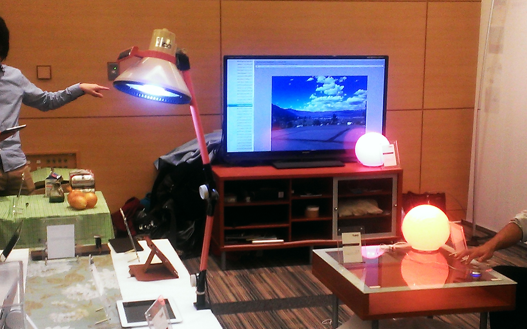
\includegraphics[width=70mm,bb=0 0 527 329]{figures/c520d5dfbd06c532d48d324a7019b00c.png}}
\caption{People trying Strotor at an exhibition.}
\label{exhibition}
\end{figure}

% Selecting a content only by rotating a dial is very 気持ち良い。
% 音楽ソース、ニュースソース、動画、Wikipediaなどあらゆるものをダイヤルやペダルだけで検索できる

\section*{CONCLUSIONS}

We have developed a new simple interaction method ``{\ST}'' for exploring
large hierarchical data structure.
{\ST} user can easily find an entry in a huge hierarchical database
only by using a rotating input device which can be installed at
wide range of locations where conventional keybords and switches do not fit.
We are hoping to try various implementations of {\ST} and try them at
various places like kitchens, restrooms, etc.

\small{
\bibliographystyle{plain}
\bibliography{paper}
}

\end{document}


